\documentclass[border=8pt]{standalone}
\usepackage{amsmath,amssymb,bm}
\usepackage{xcolor}
\usepackage{tikz}
\definecolor{P}{HTML}{D5772A}
\definecolor{ink}{HTML}{1B1B2F}
\colorlet{band}{P!7!white}
\colorlet{lcol}{P!18!white}
\colorlet{rule}{P!45!white}
\colorlet{Pd}{P!80!white}
\begin{document}
\large
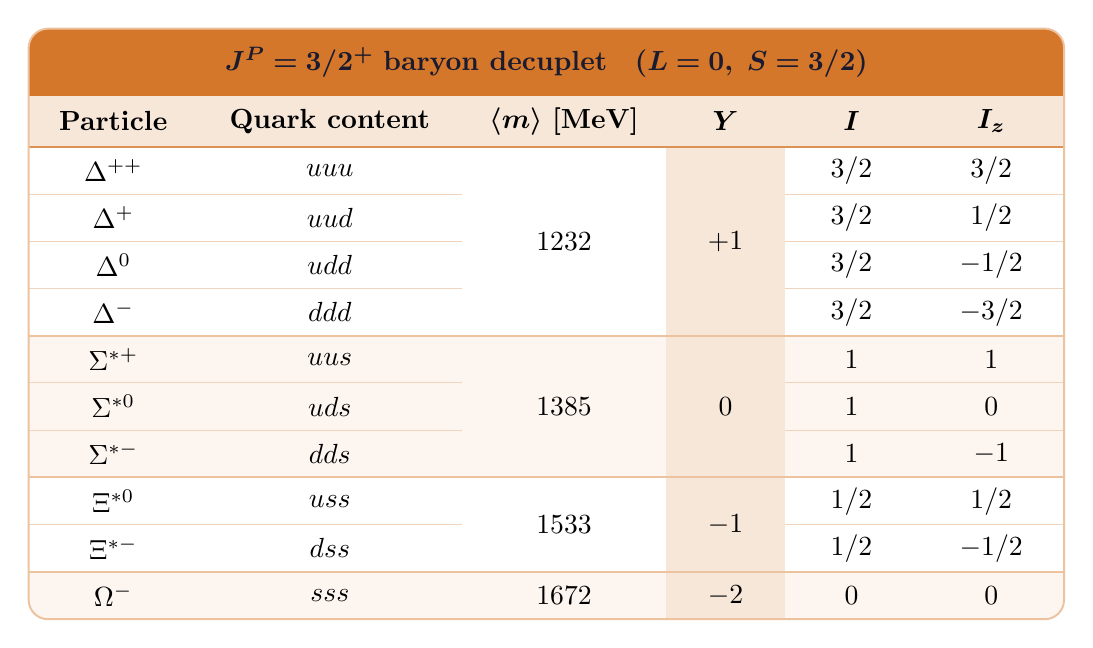
\begin{tikzpicture}
  \begin{scope}
    \clip[rounded corners=7pt] (0,0) rectangle (13.150,-7.500);
    \fill[P] (0,0) rectangle (13.150,-0.850);
    \fill[lcol] (0,-0.850) rectangle (13.150,-1.500);
    \fill[band] (0,-3.900) rectangle (13.150,-5.700);
    \fill[band] (0,-6.900) rectangle (13.150,-7.500);
    \fill[lcol] (8.100,-1.500) rectangle (9.600,-7.500);
  \end{scope}
  \draw[rule!70,line width=.35pt] (0.000,-2.100) -- (5.500,-2.100) (9.600,-2.100) -- (13.150,-2.100);
  \draw[rule!70,line width=.35pt] (0.000,-2.700) -- (5.500,-2.700) (9.600,-2.700) -- (13.150,-2.700);
  \draw[rule!70,line width=.35pt] (0.000,-3.300) -- (5.500,-3.300) (9.600,-3.300) -- (13.150,-3.300);
  \draw[rule,line width=.7pt] (0,-3.900) -- (13.150,-3.900);
  \draw[rule!70,line width=.35pt] (0.000,-4.500) -- (5.500,-4.500) (9.600,-4.500) -- (13.150,-4.500);
  \draw[rule!70,line width=.35pt] (0.000,-5.100) -- (5.500,-5.100) (9.600,-5.100) -- (13.150,-5.100);
  \draw[rule,line width=.7pt] (0,-5.700) -- (13.150,-5.700);
  \draw[rule!70,line width=.35pt] (0.000,-6.300) -- (5.500,-6.300) (9.600,-6.300) -- (13.150,-6.300);
  \draw[rule,line width=.7pt] (0,-6.900) -- (13.150,-6.900);
  \draw[Pd,line width=.7pt] (0,-1.500) -- (13.150,-1.500);
  \draw[rule,line width=.7pt,rounded corners=7pt] (0,0) rectangle (13.150,-7.500);
  \node[text=ink,align=center] at (6.575,-0.425) {$\bm{J^{P}=3/2^{+}}\ \textbf{baryon decuplet}\quad \bm{(L=0,\ S=3/2)}$};
  \node at (1.075,-1.175) {\textbf{Particle}};
  \node at (3.825,-1.175) {\textbf{Quark content}};
  \node at (6.800,-1.175) {$\bm{\langle m\rangle}$ \textbf{[MeV]}};
  \node at (8.850,-1.175) {$\bm{Y}$};
  \node at (10.450,-1.175) {$\bm{I}$};
  \node at (12.225,-1.175) {$\bm{I_z}$};
  \node at (1.075,-1.800) {$\Delta^{++}$};
  \node at (3.825,-1.800) {$uuu$};
  \node at (12.225,-1.800) {$3/2$};
  \node at (10.450,-1.800) {$3/2$};
  \node at (1.075,-2.400) {$\Delta^{+}$};
  \node at (3.825,-2.400) {$uud$};
  \node at (12.225,-2.400) {$1/2$};
  \node at (10.450,-2.400) {$3/2$};
  \node at (1.075,-3.000) {$\Delta^{0}$};
  \node at (3.825,-3.000) {$udd$};
  \node at (12.225,-3.000) {$-1/2$};
  \node at (10.450,-3.000) {$3/2$};
  \node at (1.075,-3.600) {$\Delta^{-}$};
  \node at (3.825,-3.600) {$ddd$};
  \node at (12.225,-3.600) {$-3/2$};
  \node at (10.450,-3.600) {$3/2$};
  \node at (1.075,-4.200) {$\Sigma^{*+}$};
  \node at (3.825,-4.200) {$uus$};
  \node at (12.225,-4.200) {$1$};
  \node at (10.450,-4.200) {$1$};
  \node at (1.075,-4.800) {$\Sigma^{*0}$};
  \node at (3.825,-4.800) {$uds$};
  \node at (12.225,-4.800) {$0$};
  \node at (10.450,-4.800) {$1$};
  \node at (1.075,-5.400) {$\Sigma^{*-}$};
  \node at (3.825,-5.400) {$dds$};
  \node at (12.225,-5.400) {$-1$};
  \node at (10.450,-5.400) {$1$};
  \node at (1.075,-6.000) {$\Xi^{*0}$};
  \node at (3.825,-6.000) {$uss$};
  \node at (12.225,-6.000) {$1/2$};
  \node at (10.450,-6.000) {$1/2$};
  \node at (1.075,-6.600) {$\Xi^{*-}$};
  \node at (3.825,-6.600) {$dss$};
  \node at (12.225,-6.600) {$-1/2$};
  \node at (10.450,-6.600) {$1/2$};
  \node at (1.075,-7.200) {$\Omega^{-}$};
  \node at (3.825,-7.200) {$sss$};
  \node at (12.225,-7.200) {$0$};
  \node at (10.450,-7.200) {$0$};
  \node at (8.850,-2.700) {$+1$};
  \node at (8.850,-4.800) {$0$};
  \node at (8.850,-6.300) {$-1$};
  \node at (8.850,-7.200) {$-2$};
  \node at (6.800,-2.700) {$1232$};
  \node at (6.800,-4.800) {$1385$};
  \node at (6.800,-6.300) {$1533$};
  \node at (6.800,-7.200) {$1672$};
\end{tikzpicture}
\end{document}
